\documentclass[10pt]{article}

\usepackage[utf8]{inputenc}
\usepackage[portuguese]{babel} 
\usepackage{graphicx,url}
\usepackage{amsfonts,amsmath,bm,bbm}
\usepackage{natbib}
\usepackage[colorlinks=true, allcolors=blue]{hyperref} 
\usepackage[a4paper]{geometry}
\usepackage{fourier}
\usepackage{parskip}

\sloppy

\title{Problemas Interessantes}


\author{
Eduarda T.\ C.\ Chagas\and 
Heitor S.\ Ramos\and 
Alejandro C.\ Frery\and 
Osvaldo A.\ Rosso
}


\begin{document}

\maketitle

\section{Estudo de padrões ordinais com grafos de transição e Cadeias de Markov} \label{abstract}

Uma das limitações das técnicas de análise de séries temporais baseadas em padrões ordinais é não permitirem fazer previsões (\textit{forecast}) nem simulações.
Este trabalho explora essa possibilidade.

Sejam $\bm Z=(Z_1,\dots,Z_n)$ uma série temporal de valores reais,
$\bm \pi^{(D,\tau)} = (\pi^{(D,\tau)}_1,\dots,\pi^{(D,\tau)}_{N-(D-1)\tau})$ a série de padrões a ela associados (calculados com palavras de dimensão $D$ e atraso $\tau$),
e $G=(V,E)$ o grafo de transições obtido a partir de $\bm \pi^{(D,\tau)}$.

A proposta consiste em fazer a junção das evidências de $\bm Z$, $\bm \pi^{(D,\tau)}$, e $G$ para fazer simulações e previsões a respeito da série.

O primeiro passo consiste em analisar $\bm Z$ e $\bm \pi^{(D,\tau)}$.
Para cada padrão observado em $\bm \pi^{(D,\tau)}$, serão coletados os dados que o originaram em $\bm Z$.
Consideremos, por exemplo, o caso do padrão $\pi^{(3,1)}_1=b_{j}b_{j+1}b_{j+2}$, e suponhamos que ele corresponde a todas as palavras que satisfazem $z_{j}<z_{j+1}<z_{j+2}$.
Todas essas palavras serão coletadas e analisadas para obter:
\begin{itemize}
	\item uma estimativa da distribuição três-variada, ou
	\item estimativas do valor central e estimativas de uma medida de dispersão de cada um dos três valores, por exemplo a média e o desvio padrão.
\end{itemize} 
Teremos, assim, associados ao padrão $\pi^{(3,1)}_1$, 
\begin{itemize}
	\item um modelo $\widehat{\mathcal{D}}(\pi^{(3,1)}_1)$, ou
	\item três médias $\widehat\mu_{b_j}, \widehat\mu_{b_{j+1}}, \widehat\mu_{b_{j+2}}$ e três desvios padrão $s_{b_j}, s_{b_{j+1}}, s_{b_{j+2}}$.
\end{itemize} 

O segundo passo consiste em formar a matriz de transições do grafo $G$, digamos $M$.
Por construção, a cadeia é irredutível, e basta com que haja uma única transição entre estados iguais para que a cadeia seja aperiódica.
Com estas propriedades, há uma única distribuição de equilíbrio $\Pi$, que é a solução de $\Pi M=\Pi$.

Dada a série temporal $\bm Z=(Z_1,\dots,Z_n)$, associada à sequência $\bm \pi^{(D,\tau)} = (\pi^{(D,\tau)}_1,\dots,\pi^{(D,\tau)}_{N-(D-1)\tau})$ de padrões, simularemos o evento $Z_{n+1}$ com dois elementos:
\begin{itemize}
	\item o padrão $\pi^{(D,\tau)}_1,\dots,\pi^{(D,\tau)}_{N-(D-1)\tau+1}$ que possui probabilidade máxima de ocorrência em $\Pi$ após o último padrão, e
	\item uma observação do modelo $\mathcal D$ correspondente a esse padrão. Note-se que será necessário obter apenas uma amostra da distribuição marginal de $\mathcal D$ dadas as observações já presentes nos últimos estágios da série.
\end{itemize} 

A nossa previsão da observação que sucede $Z_n$ será o estado de equilíbrio mais plausível que segue ao último padrão que inclui $Z_n$, e em cada posição do padrão colocaremos a estimativa de centralidade, munida da sua estimativa de precisão.
De forma mais sofisticada, poderemos usar o algoritmo EM~\citep{dempster_em}.

\section{Desvios do Ponto $(1,0)$}

Seja $\bm x=(x_1,x_2,\dots,x_n)$ uma sequência de observações de variáveis aleatórias independentes e identicamente distribuídas segundo uma lei $\mathcal U(0,1)$, e $\bm \pi = \big( \pi^D_1,\pi^D_2,\dots,\pi^D_{n-D+1} \big)$ a sequência de padrões ordinais de $\bm x$ e dimensão $D$.
Seja ainda $\bm h(\bm \pi)=\big(h_1,h_2,\dots,h_{D!}\big)$ o histograma de proporções dos padrões $\bm \pi$.

A entropia de Shannon do histograma de proporções $\bm h$
\begin{equation}
	H\big(\bm h(\bm \pi)\big) = -\frac{1}{\ln D!} \sum_{\ell=1}^{D!} h_\ell \ln h_\ell .
	\label{eq:entropia}
\end{equation}

Utilizaremos como distribuição de equilíbrio a lei uniforme sobre o conjunto $\{1,2,\dots,D!\}$, que é caracterizada pelas probabilidades $\bm u =\begin{pmatrix}
1/D! &1/D! &\cdots &1/D!
\end{pmatrix} $.
Denotaremos $u=1/D!$.
A entropia de $\bm u$ é $H(\bm u) = \ln D! = -\ln u$.

A distância de Jensen-Shannon entre $\bm h(\pi)$ e $\bm u$ é 
\begin{equation}
	Q'\big(\bm h(\bm \pi), \bm u\big) = H\Big(\frac{\bm h(\bm \pi) + \bm u}{2}\Big) -\frac12\big[H\big(\bm h(\bm \pi)\big) + H(\bm u)\big].
	\label{eq:distancia}
\end{equation}

Suponhamos que $h_1=u+\varepsilon$, $h_2=u-\varepsilon$, com $0\leq\varepsilon\leq u$, e que $h_\ell=u$ para todo $\ell\geq 3$.
Com essa hipótese
\begin{equation}
	\frac{\bm h(\bm \pi) + \bm u}{2} =
	\begin{pmatrix}
	u+\frac{\varepsilon}{2}
	& u-\frac{\varepsilon}{2}
	& u
	& u
	& \cdots
	& u
	\end{pmatrix} .
	\label{hu2}
\end{equation}

Verificamos que
\begin{align}
	H(\bm u) &= 1, \text{ e que}\\
	H\big(h(\bm \pi)\big) & = 
\frac{1}{\ln u} \big(	(u+\varepsilon ) \ln (u+\varepsilon )
	+ (u-\varepsilon ) \ln (u-\varepsilon )\big) +
	(1-2u) . 
	\label{eq:entropiahepsilon}
\end{align}
Assim, temos
\begin{equation}
\begin{split}
Q'\big(\bm h(\bm \pi), \bm u\big) & =
\frac{1}{2} \Bigg(
(u+\varepsilon ) \ln (u+\varepsilon )
+(u-\varepsilon ) \ln (u-\varepsilon )
+(1-2 u) \ln u
+\ln u\\
& \quad\mbox{}
- (2 u+\varepsilon ) \ln\left(u+\frac{\varepsilon }{2}\right)
-(2 u-\varepsilon) \ln \left(u-\frac{\varepsilon }{2}\right)  
\Bigg)	.
\end{split}
\label{eq:distanciaepsilon}
\end{equation}

Com~\eqref{eq:entropiahepsilon} e~\eqref{eq:distanciaepsilon} calculamos a complexidade estatística
\begin{equation}
	C\big(\bm h(\bm \pi), \bm u\big) = \frac{1}{\ln D}H\big(\bm h(\bm \pi)\big) Q'\big(\bm{h}(\bm \pi), \bm{u}\big).
	\label{eq:complexidade}
\end{equation}

A Fig.~\ref{fig:Deviations} mostra os desvios do ponto $(1,0)$, para $D=3,4,5,6$, e variações de $\varepsilon$ entre $0$ e $1/D!$.

\begin{figure}[hbt]
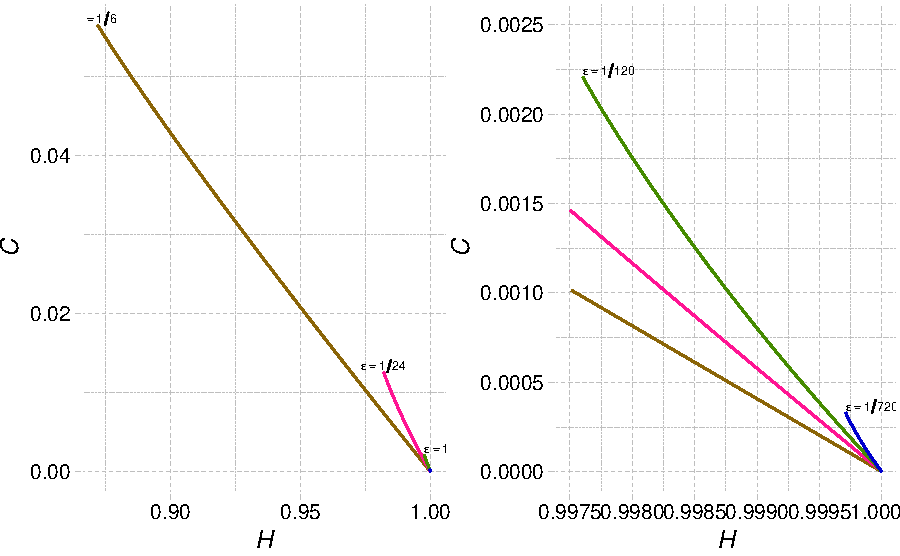
\includegraphics[width=\linewidth]{Deviations}
\caption{Desvios do ponto $(0,1)$ ao considerar que um par de bins foi alterado, para $D=3,4,5,6$.}
\label{fig:Deviations}
\end{figure}

\bibliographystyle{agsm}
\bibliography{art81,art77}

\end{document}